\documentclass{article}
\usepackage[utf8]{inputenc}

% Page setup
\usepackage[a4paper,landscape,margin=2cm]{geometry}
\usepackage{amsmath}

% Typography
\usepackage[scaled]{helvet}
\let\familydefault\sfdefault

\usepackage[usenames,svgnames]{xcolor}
\usepackage{tikz,pgfplots}
\usetikzlibrary{positioning,arrows,intersections}

\definecolor{colordelta}    {RGB}{199,212,104}
\definecolor{colorsnapshot} {RGB}{79 ,142,209}
\definecolor{colordict}     {RGB}{143,232,186}
\definecolor{colorhdt}      {RGB}{49 ,167,226}
\definecolor{colortext}     {RGB}{29 ,29 ,27 }

\begin{document}
\pagestyle{empty}
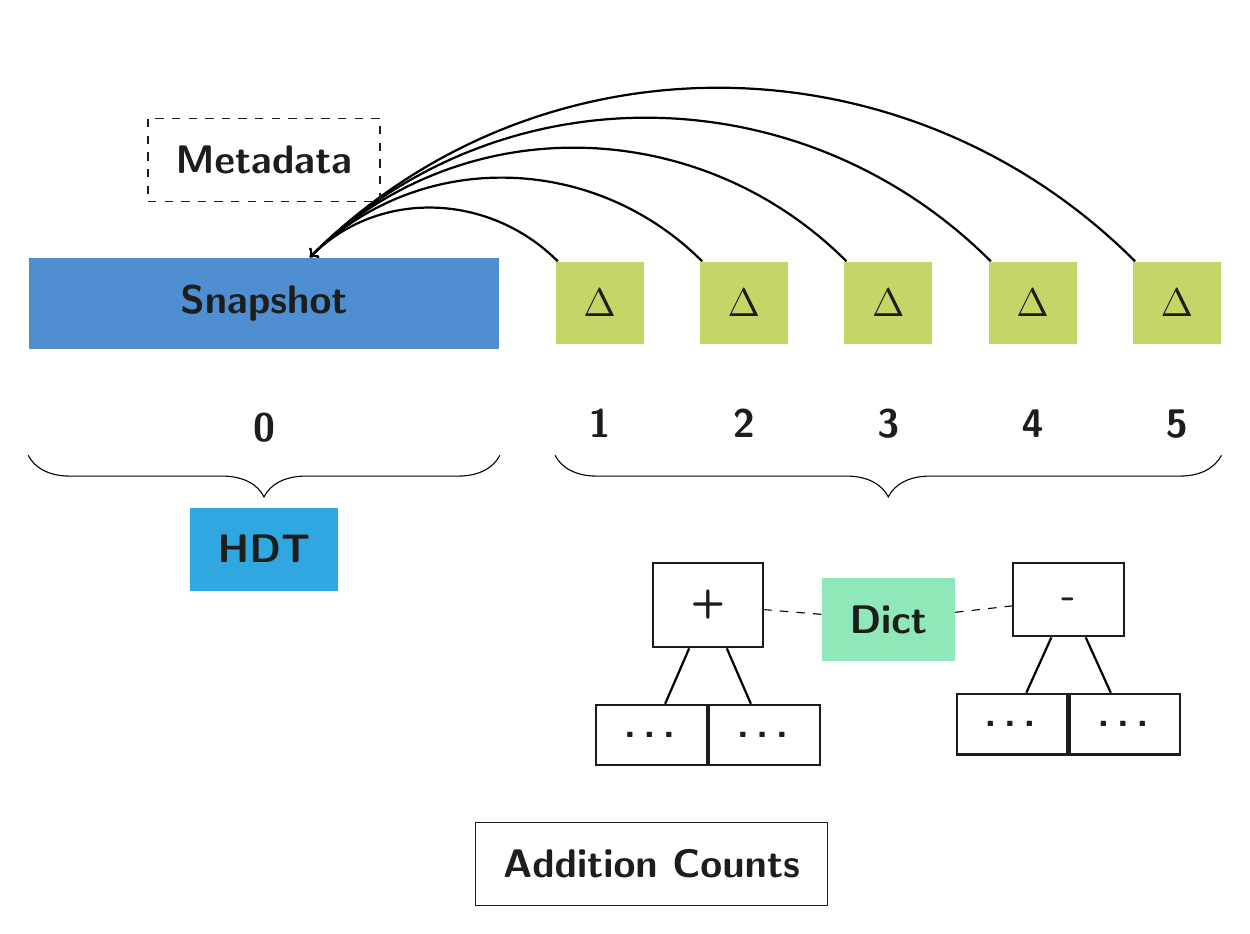
\begin{tikzpicture}[
    node distance = 2em, auto,
    font={\Large\itshape},
    base/.style={text=colortext,font={\Large\bfseries},inner sep=10pt,align=center,rectangle},
    txt/.style={text=colortext,font={\Large\bfseries},align=center},
    treenode/.style={base,thick,draw=colortext,text width=2em},
    relation/.style={text width=13em},
]

    % Nodes
    \node[base,fill=colorsnapshot,text width=15em] (snapshot) {Snapshot};
    \node[base,fill=colordelta,right=of snapshot]  (delta1)   {$\Delta$};
    \node[base,fill=colordelta,right=of delta1]    (delta2)   {$\Delta$};
    \node[base,fill=colordelta,right=of delta2]    (delta3)   {$\Delta$};
    \node[base,fill=colordelta,right=of delta3]    (delta4)   {$\Delta$};
    \node[base,fill=colordelta,right=of delta4]    (delta5)   {$\Delta$};
    
    % Text
    \node[txt,below=of snapshot] (snaptxt) {0};
    \node[txt,below=of delta1]             {1};
    \node[txt,below=of delta2]             {2};
    \node[txt,below=of delta3] (delta3txt) {3};
    \node[txt,below=of delta4]             {4};
    \node[txt,below=of delta5]             {5};
    
    % Arrows
    \draw[->,thick](delta1) to [out=135,in=45] (snapshot);
    \draw[->,thick](delta2) to [out=135,in=45] (snapshot);
    \draw[->,thick](delta3) to [out=135,in=45] (snapshot);
    \draw[->,thick](delta4) to [out=135,in=45] (snapshot);
    \draw[->,thick](delta5) to [out=135,in=45] (snapshot);
    
    % Brace around snapshot and delta's
    \draw [decorate, decoration={brace,mirror,amplitude=15pt,raise=55pt}] (snapshot.west) -- (snapshot.east);
    \draw [decorate, decoration={brace,mirror,amplitude=15pt,raise=55pt}] (delta1.west) -- (delta5.east);
    
    % Dummy nodes for spacing
    \node[below=of delta3txt.south] (trees)      {};
    \node[left=of trees]            (treesleft)  {};
    \node[right=of trees]           (treesright) {};
    
    % Additions tree
    \node[treenode,below left=of treesleft] (additionsroot)        {+};
    \node[treenode,below=of additionsroot.south west] (additions1) {\ldots};
    \node[treenode,below=of additionsroot.south east] (additions2) {\ldots};
    \draw[-,thick](additions1) -- (additionsroot);
    \draw[-,thick](additions2) -- (additionsroot);
    
    % Deletions tree
    \node[treenode,below right=of treesright] (deletionsroot)      {-};
    \node[treenode,below=of deletionsroot.south west] (deletions1) {\ldots};
    \node[treenode,below=of deletionsroot.south east] (deletions2) {\ldots};
    \draw[-,thick](deletions1) -- (deletionsroot);
    \draw[-,thick](deletions2) -- (deletionsroot);
    
    % Dictionary
    \node[base,fill=colordict,below=of trees] (dict) {Dict};
    \draw[-,dashed](dict) -- (additionsroot);
    \draw[-,dashed](dict) -- (deletionsroot);
    
    % HDT
    \node[base,fill=colorhdt,below=of snaptxt] (hdt) {HDT};
    
    % Addition Counts
    \node[base,draw=colortext,below=of additions1] (acounts) {Addition Counts};
    
    % Metadata
    \node[base,dashed,draw=colortext,above=of snapshot] (meta) {Metadata};

\end{tikzpicture}
\end{document}
